\begin{figure}[ht]
\ffigbox
	{\begin{subfigure}[b]{0.48\linewidth}
		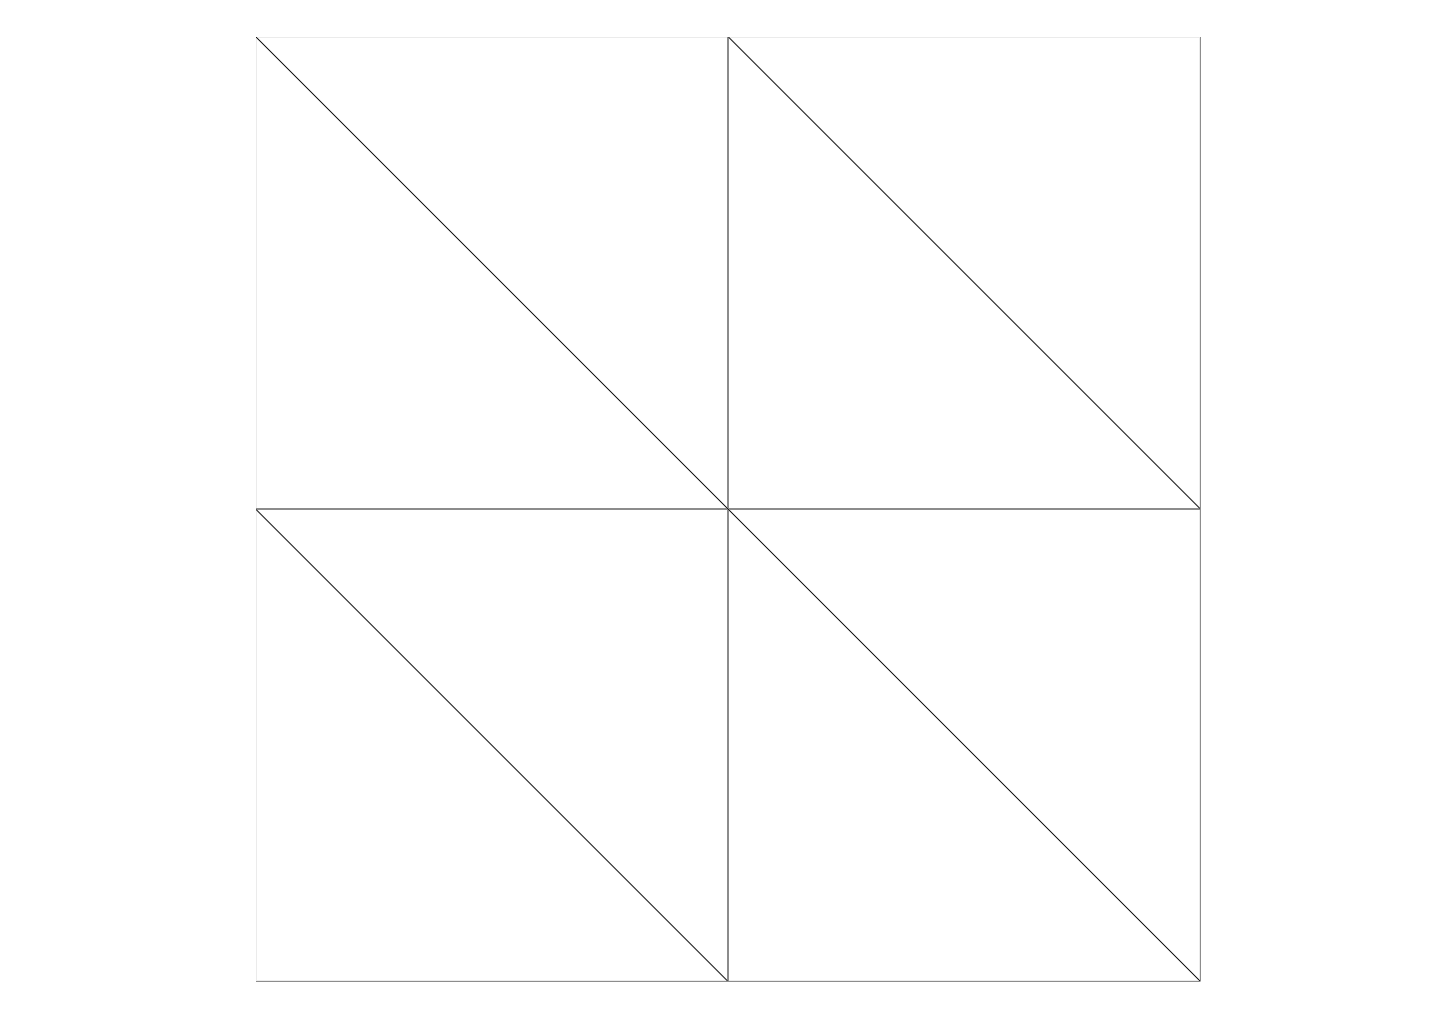
\includegraphics[width=1.0\linewidth,height=0.32\textheight,keepaspectratio]
			{data/synthetic_meshes/square_tesselation_2tri_Dirac_delta_1_v9_f8_wireframe.png}
		\caption{Sq2 v9\_f8 wireframe}\label{fig:sq2.a}
	\end{subfigure}
	\begin{subfigure}[b]{0.48\linewidth}
		
\includegraphics[width=1.0\linewidth,height=0.32\textheight,keepaspectratio]
		{data/synthetic_meshes/square_tesselation_2tri_Dirac_delta_10_v441_f800_wireframe.png}
		\caption{Sq2 v441\_f800 wireframe}\label{fig:sq2.b}
	\end{subfigure}

	\bigskip
	\begin{subfigure}[b]{0.48\linewidth}
		
\includegraphics[width=1.0\linewidth,height=0.32\textheight,keepaspectratio]
		{data/synthetic_meshes/square_tesselation_2tri_Dirac_delta_1_v9_f8_funcvals_0iter_crop.png}
		\caption{Sq2 v9\_f8 iter 0}\label{fig:sq2.c}
	\end{subfigure}
	\begin{subfigure}[b]{0.48\linewidth}
		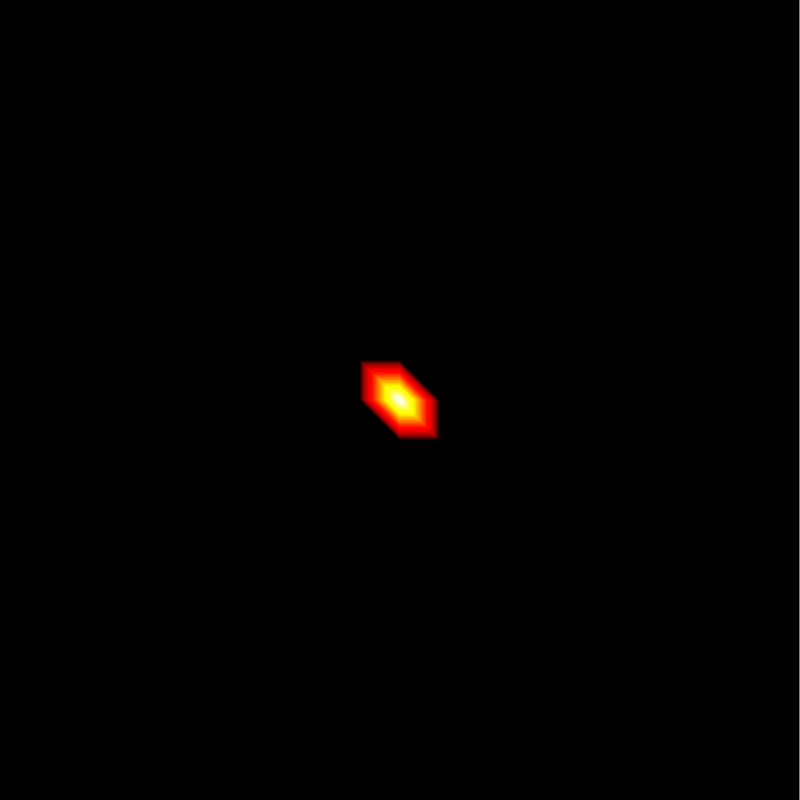
\includegraphics[width=1.0\linewidth,height=0.32\textheight,keepaspectratio]
		{data/synthetic_meshes/square_tessellation_2tri_Dirac_delta_10_v441_f800_funcvals_0iter.png}
		\caption{Sq2 v441\_f800 iter 0}\label{fig:sq2.d}
	\end{subfigure}

	\bigskip
	\begin{subfigure}[b]{0.48\linewidth}
		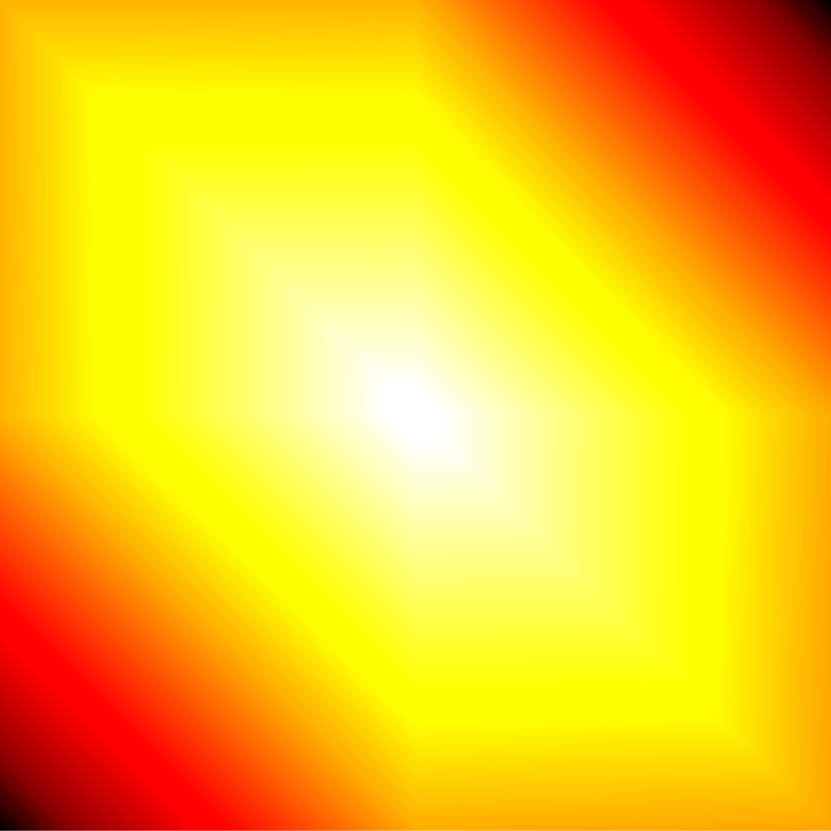
\includegraphics[width=1.0\linewidth,height=0.32\textheight,keepaspectratio]
		{data/synthetic_meshes/square_tesselation_2tri_Dirac_delta_1_v9_f8_funcvals_1iter_crop.png}
		\caption{Sq2 v9\_f8 iter 1}\label{fig:sq2.e}
	\end{subfigure}
	\begin{subfigure}[b]{0.48\linewidth}
		
\includegraphics[width=1.0\linewidth,height=0.32\textheight,keepaspectratio]
		{data/synthetic_meshes/square_tessellation_2tri_Dirac_delta_10_v441_f800_funcvals_100iter.png}
		\caption{Sq2 v441\_f800 iter 100}\label{fig:sq2.f}
	\end{subfigure}}
	{\caption[Synthetic Square, 2 triangles, Dirac delta function]{A synthetic square, subdivided by triangles, with a Dirac delta function applied: (a) wireframe (b) colored by function value before filter (c) colored by function value after 1000 iterations
%GigaMesh~\cite{Mara10} with function values colored with the Improved Hot colorramp, exported as png after disabling the background grid [f7], maximizing the window, disabling screenshot cropping, as well as rejecting tiled rendering, finally cropping to content in GIMP.
	}\label{fig:sq2}}
\end{figure}
